% Created 2024-07-31 Wed 16:04
% Intended LaTeX compiler: pdflatex
\documentclass[11pt]{article}
\usepackage[utf8]{inputenc}
\usepackage[T1]{fontenc}
\usepackage{graphicx}
\usepackage{longtable}
\usepackage{wrapfig}
\usepackage{rotating}
\usepackage[normalem]{ulem}
\usepackage{amsmath}
\usepackage{amssymb}
\usepackage{capt-of}
\usepackage{hyperref}
\usepackage{minted}
\usepackage{xcolor}
\usepackage{hyperref}
\usepackage{tocloft}
\usepackage[margin=1in]{geometry}
\usepackage{fancyhdr}
\usepackage{fancyheadings}
\usepackage{titlepic}
\usepackage{pdfpages}
\usepackage[T1]{fontenc}
\usepackage{helvet}
\usepackage{fontawesome}
\usepackage[colorlinks=true, urlcolor=blue, linkcolor=blue]{hyperref}
\usepackage{graphicx}
\usepackage[mmddyyyy]{datetime}
\setlength{\parskip}{2mm}
\setlength{\parindent}{0mm}
\setcounter{secnumdepth}{3}
\setcounter{tocdepth}{3}
\usepackage{setspace}
\usepackage{wrapfig}
\hypersetup{breaklinks=true}
\usepackage{verbatim}
\usepackage{fvextra}
\usepackage{float}
\usepackage{lipsum}
\usepackage{xurl}
\author{Hilduara Abreu}
\date{July 31, 2024}
\title{Staff Handbook 2023-2024}
\hypersetup{
 pdfauthor={Hilduara Abreu},
 pdftitle={Staff Handbook 2023-2024},
 pdfkeywords={},
 pdfsubject={},
 pdfcreator={Emacs 29.4 (Org mode 9.6.15)}, 
 pdflang={English}}
\begin{document}

\maketitle
\tableofcontents


\section{Cover Page}
\label{sec:orga5c3105}
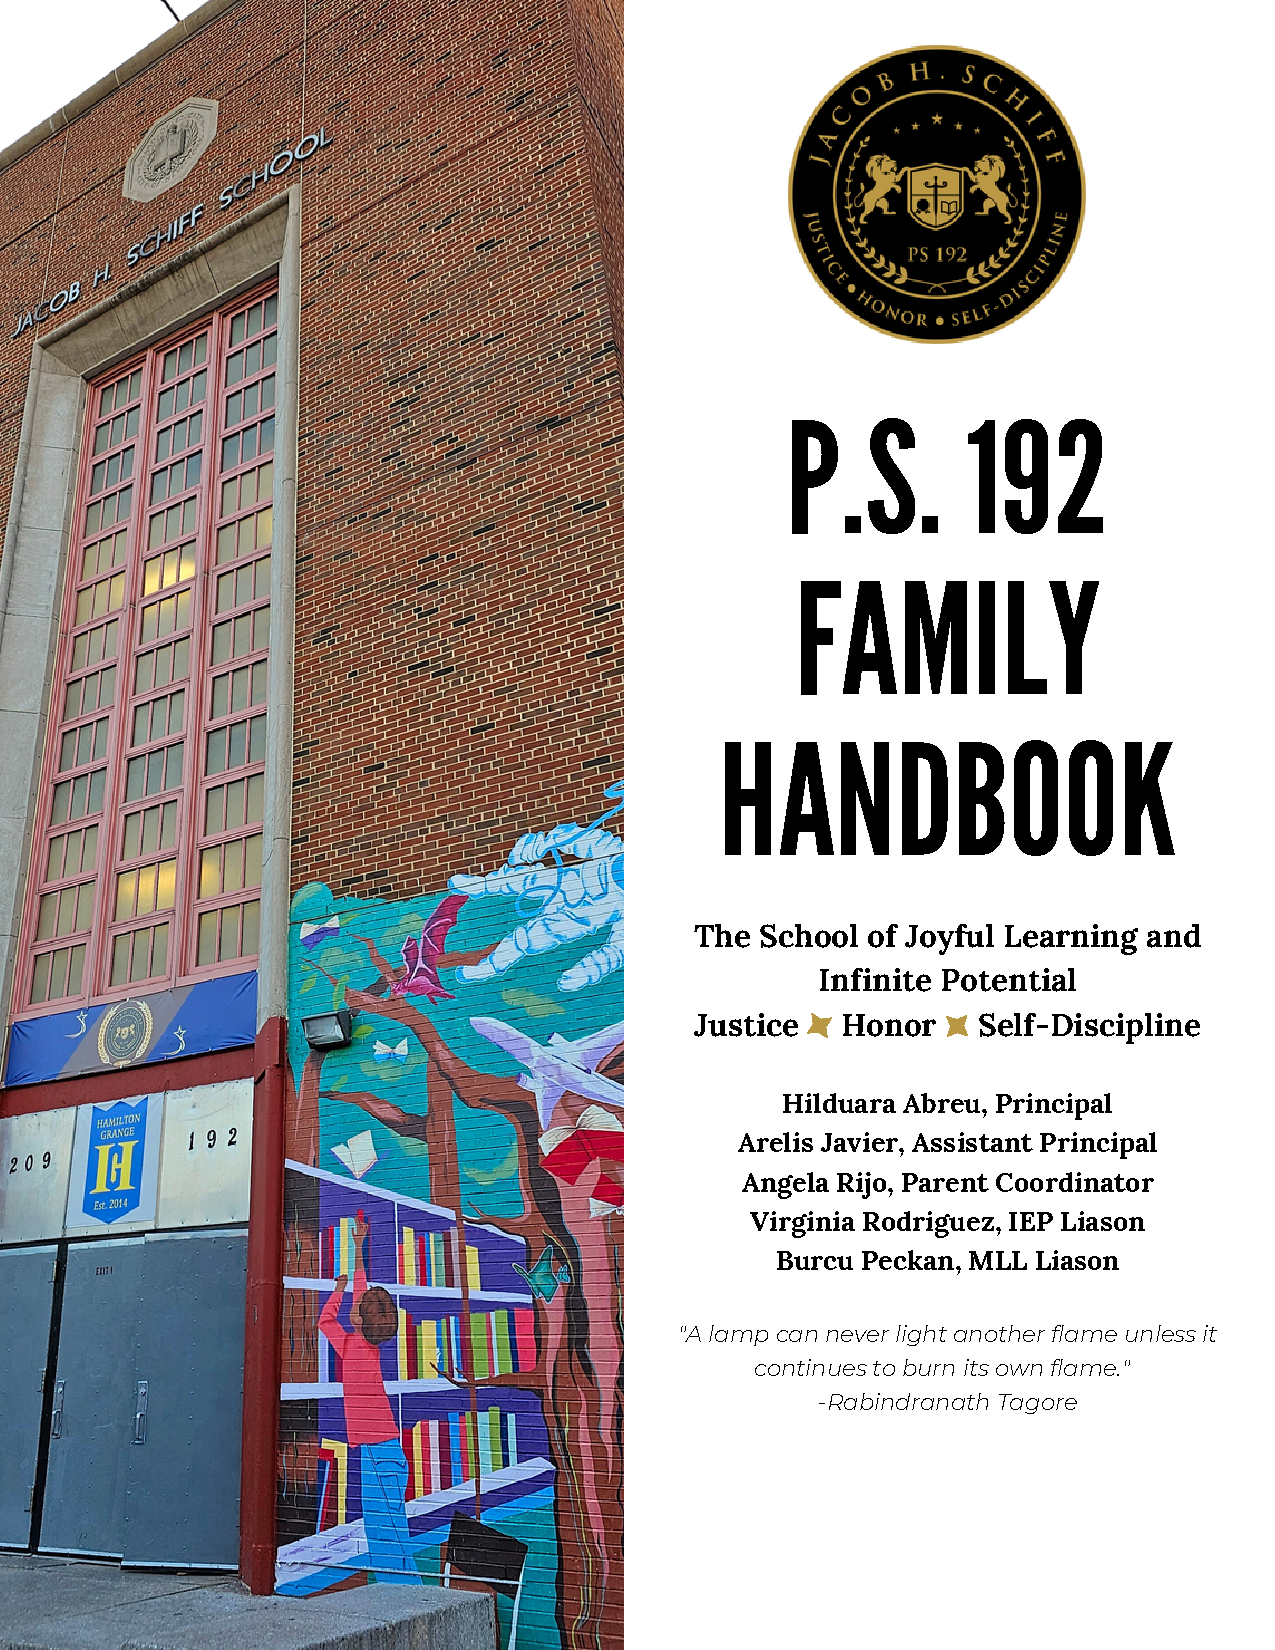
\includepdf[pages=1,fitpaper]{/home/rob/ps192_welcome_letters/2024/Welcome_Letters-En/handbook_front.pdf}

\section{Message from The Principal}
\label{sec:org4966fc0}

Welcome to \href{https://www.ps192.org}{P.S. 192}, where excellence in education is not just a goal, but a way of life. It is with immense pleasure and pride that I extend my warmest greetings to you all as we embark on yet another exciting academic year.

At \href{https://www.ps192.org}{P.S. 192}, we are more than just an educational institution; we are a community united by a shared vision of nurturing young minds and shaping future leaders. Our school's emblem, proudly displaying the noble lion and lioness, symbolizes the strength, courage, and unwavering determination that define our journey together.

As we journey forward, we remain steadfast in our commitment to instill three core values into the hearts of our students: Justice, Honor, and Self-Discipline. These values are the guiding principles that underpin everything we do. They form the bedrock upon which we build character, foster empathy, and cultivate the leaders of tomorrow.

In the pages of this Family Handbook, you will find a wealth of information about our school's policies, programs, and opportunities. It is designed to be your compass, helping you navigate the rich and rewarding educational experience we offer.

Together, as a united educational family, we will empower your child to explore their potential, embrace challenges, and emerge as confident, compassionate, and responsible individuals ready to make a positive impact on the world.

Thank you for entrusting us with the privilege of shaping your child's future. Together, we will roar with pride as our students become the lions and lionesses of tomorrow, embodying the values of justice, honor, and self-discipline.

Respectfully yours,

\begin{center}

\includegraphics[width=0.2\textwidth]{hil_signature.jpg}
\end{center}

Hilduara Abreu

Principal

\textbf{The School of Joyful Learning!}

\section{About P.S. 192 | Jacob H. Schiff School}
\label{sec:org2fd0b82}
Welcome to P.S. 192 | Jacob H. Schiff School, where we believe in nurturing "Infinite Potential" in every child. Our school is more than just a place of learning; it's a community dedicated to unlocking the limitless abilities and intelligence within each of our students through dedication, learning, and resilience. We are committed to instilling core values of justice, honor, and self-discipline in every aspect of our educational journey.

\subsection{History}
\label{sec:org897b251}
Our school was established in 1952, once home to the Hebrew Orphan Asylum of New York (HOA). It began as a modest educational institution serving the local community.

Jacob H. Schiff's contributions extended beyond our school, as he actively supported various initiatives that aimed to uplift marginalized communities, promote civil rights, and advance educational opportunities. His commitment to justice and social equity has left an enduring impact on our institution and our community.

\subsection{Our Commitment}
\label{sec:org4856e14}
At P.S. 192, we foster a dynamic and engaging learning environment. Our experienced educators are dedicated to providing personalized support to each student, recognizing that every child has unique strengths and areas for growth. We encourage curiosity, creativity, and critical thinking, empowering our students to tackle challenges as opportunities for growth and discovery.

\subsection{Core Values}
\label{sec:org3f01635}
\begin{itemize}
\item Justice: At P.S. 192, we teach our students the importance of fairness and equity. We instill a sense of social responsibility, encouraging them to be advocates for justice in their school, community, and the world.
\item Honor: We emphasize the value of integrity and respect. Our students learn the importance of honesty, trustworthiness, and treating others with dignity, ensuring they carry these principles throughout their lives.
\item Self-Discipline: Self-discipline is a cornerstone of personal growth. We guide our students in developing strong work ethics and the ability to set and achieve goals. We believe that self-discipline is the key to unlocking their infinite potential.
\end{itemize}

\subsection{Infinite Potential}
\label{sec:org2304fab}
"Infinite Potential" is not just a slogan; it's a guiding philosophy at P.S. 192 | Jacob H. Schiff School. We believe that every child possesses boundless possibilities waiting to be unlocked. By nurturing their potential and instilling the values of justice, honor, and self-discipline, we prepare them to succeed academically, socially, and morally.

\subsection{Mission}
\label{sec:org751249b}
To provide a welcoming, safe, resourceful, and nurturing environment that supports our school community's academic and social-emotional development where children are respected and engaged in challenging curricula that motivate them to realize their potential as active, lifelong learners. Through our guiding core values of Justice, Honor, and Self-discipline, we aspire to promote perseverance, love, empathy, and respect for oneself and others.

\subsection{Vision}
\label{sec:orgd8a6419}
To ensure all students acquire the essential knowledge and skills they need to become independent thinkers and become active participants and contributors in their roles as students and as members of society.

\subsection{School Motto}
\label{sec:org72be0fd}
"Good, better, best. Never let it rest until your good is better, and your better is best." | St. Jerome

\subsection{School-Wide Norms of Conduct}
\label{sec:org3f8a107}
P.S. 192 follows school-wide norms which is the daily recitation of the Positivity Pledge every morning.

\subsection{Our Teaching Staff}
\label{sec:org0ca01b5}
P.S. 192 prides itself on the quality of our teachers. Our teaching staff is diverse with a variety of skills and expertise. Teachers work together sharing talents and strengths to maximize learning and opportunities for students.

Our faculty includes 12 classroom teachers, a physical education teacher, two ENL teachers, a Science teacher, an IEP Liaison. We have two arts teachers on faculty specializing in Visual Arts and Music and bring in consultants to teach Dance and Drama. Our Social Workers and school psychologist help students with social and emotional development. We often host student teachers from City College and Columbia University’s Teachers College. Lastly, we have a robust staff of paraprofessionals speech pathologists, an occupational therapist, and a physical therapist who work with our teachers to provide individualized support.

\subsection{Looping Model \& Curricula}
\label{sec:org7e288a9}
\subsubsection{Looping Model}
\label{sec:orgc3c05fb}
Looping is a practice where a teacher stays with the same group of students for more than one school year, fostering a continuous and supportive learning environment. Here's why it's crucial for your child's education:

\begin{itemize}
\item \textbf{Strong Teacher-Student Relationships}: Looping allows teachers to develop deeper bonds with students. They understand each child's unique learning style, strengths, and areas of improvement, resulting in a more tailored educational experience.
\end{itemize}
Consistency and Stability: By staying together, students and teachers create a stable and familiar classroom environment. This reduces anxiety, encourages active participation, and enhances the overall learning experience.
\begin{itemize}
\item \textbf{Seamless Transition}: Moving from one grade to another can be challenging for children. Looping eases this transition as students remain with a familiar teacher, minimizing disruptions and ensuring a smoother academic journey.
\item \textbf{Academic Growth}: Teachers can build on the knowledge gained in the previous year, enabling a more fluid progression of skills and concepts. This often leads to improved academic outcomes.
\item \textbf{Personalized Support}: With a deeper understanding of each student's needs, looping teachers can provide targeted interventions and support, ensuring that every child reaches their full potential.
\end{itemize}

As parents, your involvement and support are vital to the success of the looping process. We encourage you to communicate regularly with your child's teacher and stay engaged in their educational journey.

\subsubsection{Curricula}
\label{sec:org44d36e3}
\textbf{Exploring the World Through Expeditionary Learning, enVision, Passport-to-Social-Studies, Amplify Science \& Sanford Harmony}

At \href{https://www.ps192.org}{P.S. 192} | Jacob H. Schiff, we are committed to providing your child with an enriching and dynamic educational experience. One of the exciting approaches we use to ignite their curiosity and love for learning is Expeditionary Learning!

\begin{itemize}
\item \textbf{Expeditionary Learning}
\begin{itemize}
\item The EL Education curriculum is founded on the principles of the Science of Reading, incorporating systematic phonics instruction to enable every student to proficiently read challenging grade-level materials and attain mastery of literacy standards, thereby ensuring equitable educational outcomes for all students.
\item Our educational program fosters profound understanding through the incorporation of content-rich, genuine texts related to real-world subjects encompassing social studies, STEM, and literature. Students utilize their acquired knowledge to advocate for social justice and environmental responsibility, concurrently cultivating virtuous attributes that empower them to make meaningful contributions to the improvement of society.
\end{itemize}

\item \textbf{Envision}
\begin{itemize}
\item This instructional tool finds application in classrooms worldwide. enVision Mathematics places its emphasis on fostering a profound conceptual grasp of mathematics through the utilization of visual models, personalized instruction, and the implementation of 3-act tasks. Additionally, Family Engagement resources are made available to offer indispensable information to families, enabling them to support their students in their home learning endeavors. Furthermore, the program offers a comprehensive vertical alignment spanning from Kindergarten through Algebra 2, enabling schools to effectively address and meet mathematical standards.
\end{itemize}

\item \textbf{Passport-to-Social-Studies}
\begin{itemize}
\item This program prompts students to adopt a historical mindset, urging them to pose inquiries, engage in critical thinking, explore various viewpoints, and amass substantiating evidence to underpin their analyses. This is achieved through the cultivation of skills in chronological analysis, decision-making, and the rigorous pursuit of historical research and examination.
\end{itemize}

\item \textbf{Amplify Science}
\begin{itemize}
\item Students assume the role of scientists or engineers as they actively explore captivating phenomena through interactive hands-on exercises, immersive digital simulations, extensive reading and writing tasks, and dynamic classroom discussions.
\end{itemize}

\item \textbf{Sanford Harmony}
\begin{itemize}
\item The socio-emotional program fosters enhanced classroom relationships, allowing educators to allocate less effort to the management of disruptive classroom conduct and dedicate more time to instruction.
\end{itemize}
\end{itemize}

\begin{center}

\includegraphics[width=1\linewidth]{1.png}
\end{center}
\end{document}
